\section{Résumé}

Cet atelier a pour but de vous faire découvrir la modélisation 3D d'une manière peu connue : uniquement avec du code.
Pour cela vous aller utiliser le logiciel \textbf{OpenSCAD}.

\vspace{10pt}

\begin{figure}[h]
	\centering
	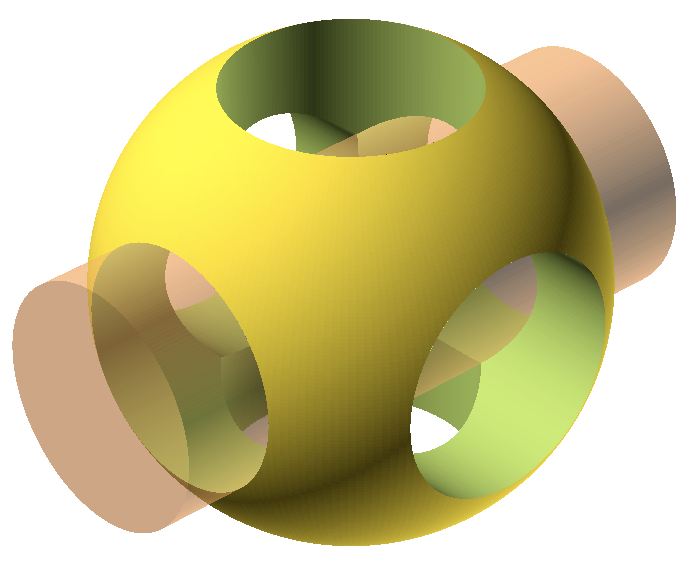
\includegraphics[width=8cm]{images/logo-openscad.png}
	\caption{\textit{Logo d'OpenScad}}
\end{figure}

\vspace{10pt}

Vous allez découvrir l'environnement de travail, comment intégrer des formes basiques et leur appliquer diverses transformations, puis vous pourrez créer vos propres modèles plus complexes.
D'ici la fin de ce sujet, vous serez en pleine mesure de modéliser l'objet de votre choix.